\documentclass[11pt,a4paper]{article}

\usepackage[T1]{fontenc}
\usepackage{newpxtext}
\usepackage[scaled=0.92]{inconsolata}
\usepackage[a4paper,margin=2.15cm,headheight=14pt]{geometry}
\usepackage{microtype}
\usepackage{graphicx}
\usepackage{booktabs}
\usepackage{tabularx}
\usepackage{array}
\usepackage{longtable}
\usepackage{colortbl}
\definecolor{thead}{gray}{0.93}
\setlength{\aboverulesep}{0.45ex}
\setlength{\belowrulesep}{0.45ex}
\setlength{\extrarowheight}{1.4pt}
\renewcommand{\arraystretch}{1.08}
\usepackage{enumitem}
\usepackage{setspace}
\usepackage{fancyhdr}
\usepackage{titlesec}
\usepackage{caption}
\usepackage{fancyvrb}
\usepackage{fvextra}
\usepackage{listings}
\usepackage[skins,breakable,listings]{tcolorbox}
\usepackage{hyperref}

\setstretch{1.07}
\setlength{\parindent}{0pt}
\setlength{\parskip}{0.42em}
\setlength{\emergencystretch}{2em}

\definecolor{codebg}{RGB}{246,246,243}
\definecolor{codeframe}{RGB}{214,214,208}
\definecolor{codebar}{RGB}{236,236,232}
\definecolor{pykw}{RGB}{22,74,122}
\definecolor{pystr}{RGB}{138,72,36}
\definecolor{pycom}{RGB}{112,112,106}
\definecolor{quiet}{RGB}{90,90,90}

\lstdefinestyle{py}{
  language=Python,
  basicstyle=\ttfamily\footnotesize\color{black!88},
  keywordstyle=\color{pykw}\bfseries,
  commentstyle=\color{pycom},
  stringstyle=\color{pystr},
  showstringspaces=false,
  columns=fullflexible,
  keepspaces=true,
  breaklines=true,
  upquote=true,
  aboveskip=0pt,
  belowskip=0pt,
  xleftmargin=2pt
}

\tcbset{enhanced,breakable}
\newtcolorbox{jsonbox}{
  colback=codebg,
  colframe=codeframe,
  boxrule=0.5pt,
  arc=2pt,
  left=8pt,right=8pt,top=6pt,bottom=6pt,
  before skip=0.55em,
  after skip=0.45em
}
\newenvironment{json}{%
  \VerbatimEnvironment
  \begin{jsonbox}%
  \begin{Verbatim}[fontsize=\footnotesize,formatcom=\color{black!88}]%
}{%
  \end{Verbatim}%
  \end{jsonbox}%
}
\newtcblisting{pycase}[2]{
  listing only,
  listing options={style=py},
  colback=codebg,
  colframe=codeframe,
  boxrule=0.5pt,
  arc=2pt,
  title={#1\hfill{\normalfont\color{pykw}#2}},
  fonttitle=\footnotesize\bfseries,
  colbacktitle=codebar,
  coltitle=black,
  toptitle=3.5pt,
  bottomtitle=3.5pt,
  left=6pt,right=6pt,top=2pt,bottom=3pt,
  before skip=0.85em,
  after skip=0.15em
}

\pagestyle{fancy}
\fancyhf{}
\fancyhead[L]{\small CS455 CodeClash}
\fancyhead[R]{\small Deliverable 2}
\renewcommand{\headrulewidth}{0.4pt}
\fancyfoot[C]{\small\thepage}
\fancypagestyle{plain}{%
  \fancyhf{}%
  \renewcommand{\headrulewidth}{0pt}%
  \fancyfoot[C]{\small\thepage}%
}

\hypersetup{
  colorlinks=true,
  linkcolor=black,
  urlcolor=black,
  pdftitle={CodeClash Deliverable 2: API, Jira and Traceability},
  pdfauthor={CS455 CodeClash team}
}

\titleformat{\section}{\Large\bfseries}{\thesection}{0.65em}{}[\vspace{0.15em}{\color{black!18}\titlerule}]
\titleformat{\subsection}{\large\bfseries}{\thesubsection}{0.55em}{}
\titlespacing*{\section}{0pt}{1.45em}{0.75em}
\titlespacing*{\subsection}{0pt}{1.15em}{0.4em}
\captionsetup{font=small,labelfont=bf,skip=0.35em}
\setlist[itemize]{leftmargin=1.15em,itemsep=0.08em,topsep=0.15em}
\setlist[enumerate]{leftmargin=1.3em,itemsep=0.1em,topsep=0.15em}
\newcolumntype{Y}{>{\raggedright\arraybackslash}X}
\fvset{fontsize=\footnotesize,breaklines,breakanywhere}

\newcommand{\meta}[1]{{\footnotesize\color{quiet}#1}\par\vspace{0.2em}}
\newcommand{\step}[1]{\par\vspace{0.45em}{\bfseries #1}\par\vspace{0.05em}}

\begin{document}

\thispagestyle{empty}
\vspace*{\fill}
\begin{center}
{\small\textsc{CS455 Project}}\\[0.85em]
{\normalsize Deliverable 2 \quad\textperiodcentered\quad Sprint 1}\\[1.7em]
{\huge\bfseries CodeClash}\\[0.6em]
{\Large API, Jira and Traceability}\\[1.15em]
{\color{black!22}\rule{3.4cm}{0.7pt}}\\[1.35em]
\begin{tabular}{@{}l@{\hspace{2.1em}}l@{}}
Ridham Divyakant Solanki & {\small\color{quiet}230853} \\[0.38em]
Peeyush Agarwal & {\small\color{quiet}230749} \\[0.38em]
Srujan Sachin Bhirud & {\small\color{quiet}231039} \\[0.38em]
Aritra Kolay & {\small\color{quiet}230192} \\[0.38em]
Om Chandrakant Chaudhari & {\small\color{quiet}230715} \\
\end{tabular}\\[1.45em]
\url{https://github.com/SrujanBhirud/CodeClash}
\end{center}
\vspace*{\fill}

\clearpage
\tableofcontents
\vspace{1em}

\section{API documentation}

The REST API runs at \url{http://localhost:4000} in local development. This section covers the 17 endpoints on \texttt{main} after pull request~\#13. The practice archive described in \S\ref{sec:archive} is the progress-demo seed on \texttt{feature/CC-52-milestone-demo}: 146 problems and 33 tags. That branch is not merged. Hidden tests are never returned by any of these routes.

\subsection{Conventions}

\begin{itemize}
\item Bodies are JSON (\texttt{Content-Type: application/json}), at most 256\,KB.
\item Authentication: send \texttt{Authorization: Bearer <access>}. Access tokens are JWTs that expire after 15 minutes. Refresh tokens last 14 days and are single use: each refresh returns a new pair.
\item Roles: \texttt{participant}, \texttt{setter}, \texttt{organiser}, \texttt{admin}. Every role check runs on the server.
\item Email confirmation: a new account starts unconfirmed. Run and practice submit answer 403 until the address is confirmed.
\item Errors always have the shape \texttt{\{"error": "<message>"\}}.
\end{itemize}

\begin{center}
\small
\begin{tabularx}{\textwidth}{@{}l Y@{}}
\toprule
\rowcolor{thead} Status & When \\
\midrule
400 & Body or query failed validation, or an id is not a valid ObjectId. \\
401 & No token, an invalid or expired token, or a wrong email or password. \\
403 & Signed in but not allowed: wrong role, email not confirmed, or someone else's submission. \\
404 & The problem, version, submission, or user does not exist. \\
409 & Email already registered, email already confirmed, or an admin removing their own admin role. \\
429 & More than 10 sign-in attempts per email per minute, or more than \texttt{SUBMIT\_PER\_MINUTE} (default 12) submissions per user per minute. \\
500 & Unexpected error. Details go to the server log only. \\
\bottomrule
\end{tabularx}
\end{center}

\subsection{Endpoints}

\begin{center}
\small
\begin{tabularx}{\textwidth}{@{}l Y l@{}}
\toprule
\rowcolor{thead} Method & Path & Auth \\
\midrule
GET & \texttt{/health} & none \\
POST & \texttt{/api/auth/register} & none \\
POST & \texttt{/api/auth/login} & none \\
POST & \texttt{/api/auth/verify} & none \\
POST & \texttt{/api/auth/verify/resend} & signed in \\
POST & \texttt{/api/auth/refresh} & refresh token \\
POST & \texttt{/api/auth/logout} & refresh token \\
GET & \texttt{/api/me} & signed in \\
GET & \texttt{/api/archive} & optional \\
GET & \texttt{/api/archive/:problemId} & none \\
GET & \texttt{/api/problem-versions/:id/public} & none \\
POST & \texttt{/api/run} & signed in, email confirmed \\
POST & \texttt{/api/practice/submissions} & signed in, email confirmed \\
GET & \texttt{/api/submissions/:id} & owner or admin \\
GET & \texttt{/api/admin/users} & admin \\
PUT & \texttt{/api/admin/users/:id/role} & admin, audited \\
GET & \texttt{/api/admin/audit} & admin \\
\bottomrule
\end{tabularx}
\end{center}

The first fourteen routes are on both \texttt{main} and the progress-demo branch. The three admin routes arrived with CC-34 and are on \texttt{main} only.

\subsection{Health}

\texttt{GET /health} pings MongoDB and Redis and needs no token.

\begin{json}
{ "ok": true, "mongo": true, "redis": true }
\end{json}

\subsection{Accounts and sessions (CC-17)}

\texttt{POST /api/auth/register} creates a participant and returns a session (201). Outside production the response also carries \texttt{verifyToken}, because local development has no mail server. It returns 409 if the email is already registered. Passwords are hashed with Argon2id.

\begin{json}
{ "email": "neha@example.com", "password": "at-least-8-chars",
  "displayName": "Neha" }
\end{json}

\begin{json}
{ "access": "<jwt>", "refresh": "<opaque>",
  "user": { "id": "...", "role": "participant",
            "displayName": "Neha", "emailVerified": false,
            "rating": 1200 },
  "verifyToken": "<dev only>" }
\end{json}

\texttt{POST /api/auth/login} takes \texttt{\{email, password\}} and returns \texttt{\{access, refresh, user\}} (200). It returns 401 on a wrong email or password, and 429 after 10 attempts for one email within a minute.

\texttt{POST /api/auth/verify} takes \texttt{\{"token": "<verifyToken>"\}} and returns \texttt{\{id, emailVerified: true\}}. It returns 400 if the token is unknown or older than 24 hours.

\texttt{POST /api/auth/verify/resend} (signed in) issues a new confirmation token and returns \texttt{\{"sent": true\}}, plus \texttt{verifyToken} outside production. It returns 409 if the email is already confirmed.

\texttt{POST /api/auth/refresh} takes \texttt{\{"refresh": "<opaque>"\}} and returns a new \texttt{\{access, refresh, user\}}. The old refresh token stops working. Presenting a refresh token that was already used revokes every token from that sign-in and returns 401.

\texttt{POST /api/auth/logout} takes \texttt{\{"refresh": "<opaque>"\}}, revokes that token, and returns 204.

\texttt{GET /api/me} (signed in) returns \texttt{\{id, role, displayName, email, emailVerified, rating\}}. There is no route that writes the profile.

\subsection{Practice archive (CC-26)}
\label{sec:archive}

\texttt{GET /api/archive} lists the latest published version of each problem. Signing in is optional. When the caller is signed in, each row also carries that caller's own status.

\begin{center}
\small
\begin{tabularx}{\textwidth}{@{}l l Y@{}}
\toprule
\rowcolor{thead} Query & Default & Meaning \\
\midrule
\texttt{q} & empty & Case-insensitive match on the title. \\
\texttt{tag} & empty & Exact tag. \\
\texttt{difficulty} & empty & \texttt{easy}, \texttt{medium}, or \texttt{hard}. \\
\texttt{status} & empty & \texttt{solved}, \texttt{attempted}, or \texttt{unsolved}. \\
\texttt{page} & 1 & Page number, from 1. \\
\texttt{pageSize} & 50 & 1 to 100. \\
\bottomrule
\end{tabularx}
\end{center}

On the progress-demo seed the unfiltered \texttt{total} is 146: 26 problems written for the archive, and 120 public Codeforces problems from the DeepMind CodeContests set. Each Codeforces row has a \texttt{source} such as \texttt{Codeforces 519B}. Difficulties are easy (67), medium (53), and hard (26). \texttt{tags} is the 33 tag names, most used first. The first twelve are math, implementation, greedy, dp, brute-force, data-structures, sortings, strings, bitmasks, combinatorics, graphs, and binary-search. Twenty-one tags follow those. A tag or difficulty filter changes \texttt{total} to the size of that subset. \texttt{solvedCount} and \texttt{acceptance} are zero or null until someone has a judged submission.

\begin{json}
{ "items": [{
    "problemId": "...", "versionId": "...",
    "title": "A and B and Compilation Errors",
    "tags": ["data-structures", "implementation", "sortings"],
    "difficulty": "easy", "rating": 1100,
    "source": "Codeforces 519B",
    "acceptance": null, "solvedCount": 0,
    "status": "unsolved" }],
  "total": 146, "page": 1, "pageSize": 50,
  "tags": ["math", "implementation", "greedy", "..."] }
\end{json}

\texttt{GET /api/archive/:problemId} returns \texttt{\{problemId, versionId, title, statement, samples, editorial\}} for the latest published version, or 404 if the problem has none.

\texttt{GET /api/problem-versions/:id/public} returns \texttt{\{problemId, versionId, title, statement, samples, tags, difficulty, limits, editorial\}}, or 404 unless that version is published.

\subsection{Running and submitting code (CC-26, CC-27)}

The languages are \texttt{python} (Python~3) and \texttt{javascript} (Node). Unless the problem stores its own limits, each test gets 2000\,ms and 256\,MB. C, C++17, Java, and Go are not accepted.

\texttt{POST /api/run} (signed in, email confirmed) runs the visible sample tests in the sandbox and stores nothing. It returns one result per sample, with stdout cut to 2000 characters, or 400 if the problem has no sample tests.

\begin{json}
{ "problemVersionId": "...", "language": "python",
  "code": "print(sum(map(int, input().split())))" }

{ "results": [{ "verdict": "AC", "stdout": "3\n" }] }
\end{json}

\texttt{POST /api/practice/submissions} (signed in, email confirmed) queues a submission against the hidden tests and answers at once. A judge worker decides the verdict. It takes the same body as \texttt{/api/run}. An optional \texttt{Idempotency-Key} header, at most 80 characters, makes a resend return the first submission instead of creating another. The submission is judged against the version id in the body.

\begin{center}
\small
\begin{tabularx}{\textwidth}{@{}l l Y@{}}
\toprule
\rowcolor{thead} Status & Body & Meaning \\
\midrule
202 & \texttt{\{"id", "replay": false\}} & Saved as queued and added to the Redis stream. \\
200 & \texttt{\{"id", "replay": true\}} & Same idempotency key as an earlier submission. Nothing new was queued. \\
\bottomrule
\end{tabularx}
\end{center}

\texttt{GET /api/submissions/:id} (signed in) is polled until \texttt{status} is \texttt{judged}. Only the owner or an admin may read it. Anyone else gets 403.

\begin{json}
{ "id": "...", "status": "judged",
  "verdict": "TLE", "reason": "time limit" }
\end{json}

\texttt{status} moves \texttt{queued} $\rightarrow$ \texttt{claimed} $\rightarrow$ \texttt{running} $\rightarrow$ \texttt{judged}. \texttt{verdict} is null until then, and then one of AC, WA, TLE, MLE, RE, or CE. \texttt{reason} is \texttt{time limit}, \texttt{memory limit}, \texttt{output limit}, or the first 500 characters of stderr for RE and CE, and null for AC and WA.

\subsection{How a verdict is committed exactly once}

\begin{enumerate}
\item The API inserts the submission as queued, then calls \texttt{XADD} on the stream.
\item A judge worker reads the stream through the consumer group \texttt{judges} and claims the submission with a fresh random \texttt{claimToken}.
\item The worker saves the verdict with an update whose filter matches both the submission id and its own token.
\item If a worker dies, \texttt{XAUTOCLAIM} gives the entry to another worker after 60 seconds of idleness. That worker writes a new token, so a late commit by the first worker matches nothing.
\item A submission still queued after 2 minutes is added to the stream again by the API, which covers a save made while Redis was down.
\end{enumerate}

The test \texttt{ignores a stale claim token and commits one verdict} is in \texttt{server/src/domain/domain.test.ts}.

\subsection{Administration (CC-34, pull request \#13)}

All three endpoints need the admin role. Anyone else gets 403. These routes are on \texttt{main}. They are not on the progress-demo branch, which was cut before this merge.

\texttt{GET /api/admin/users} returns the 50 newest accounts as \texttt{[\{id, email, displayName, role\}]}.

\texttt{PUT /api/admin/users/:id/role} takes \texttt{\{"role": "setter"\}} and returns \texttt{\{"role": "setter"\}}. The change is written to the append-only audit database. It returns 409 if an admin tries to remove their own admin role, and 404 if the user does not exist.

\texttt{GET /api/admin/audit} returns the 100 newest audit rows, newest first. The audit database user may only find and insert, so the application cannot change or delete these rows.

\begin{json}
[{ "_id": "...", "actor": "<admin id>", "actorType": "user",
   "action": "user.role", "target": "<user id>",
   "decision": "setter",
   "payload": { "before": null, "after": null, "reason": "" },
   "at": "2026-10-15T16:31:59.000Z" }]
\end{json}

\section{Jira sprint board and development history}

Sprint~1 is closed. What landed on \texttt{main} is the path we could actually finish: the local stack, the workspace layout, CI, sign-in, the sandbox, a practice submission, exactly-once judging, and the audit log. \#13 (CC-34) is the last of those merges.

The goal we had written for the sprint was ahead of that path. Seat reservation needs a contest to reserve a seat in, and contest setup was not something this sprint could start, so seats stayed with the contest work in Sprint~2. The ``policy gate'' in the same sentence turned out, once we built privileged actions, to be the audit log: the action is written down, and that record cannot be edited. The goal text on the board still has the earlier wording. The issues that closed are the ones above.

\subsection{Sprint 1 on the board}

\begin{center}
\small
\begin{tabularx}{\textwidth}{@{}l Y@{}}
\toprule
\rowcolor{thead} Item & Value \\
\midrule
Board & Jira project CC, board 1, \url{https://cs455-codeclash.atlassian.net} \\
Sprint goal & Sign-in, a judged submission, the claim-token commit, and an audit of privileged actions. Seats moved out with contest setup. \\
Deliverable~1 window & 28 September to 14 October, 31 planned points. \\
Started in Jira & 11 October, 17:49 IST, once the repository layout was in place. \\
Planned end & 14 October, 18:00 IST. \\
Closed in Jira & 15 October, 21:33 IST. CC-34's merge, which Deliverable~1 uses as Done, is 22:01 the same evening. \\
Work items & 9 of 9 Done, including the sub-task CC-4. \\
Points & 31 in the Deliverable~1 plan. 43 in Jira after the estimates below were raised. \\
\bottomrule
\end{tabularx}
\end{center}

The estimates moved once the work was in front of us. The sandbox, the claim-token commit, and the audit database were each larger than the original number, so those issues were raised in Jira. The nine items are now CC-1 (3), CC-2 (4), CC-3 (3), CC-4 (3), CC-16 (5), CC-17 (4), CC-26 (5), CC-27 (8), and CC-34 (8). Deliverable~1 had planned 31 points for the sprint, with CC-4 counted inside CC-2, and that 31 is still the figure we use for velocity.

\subsection{An update after Sprint 1}

Deliverable~1 had four sprints and 86 mandatory points, and it had already taken the agents, the per-user quota, and the burst tests off that list. Building the judge showed that the later sprints were not in an order we could follow, so we updated the plan.

An escape suite and a burst script both need real problems and a judge that can run them, and authoring was not going to be ready in the sprint that had been asked to carry those scripts. Quota and the burst scripts had also found their way back into a sprint after we had taken them off the mandatory list. Sprint~2 is therefore the contest path that Sprint~1 could not start: setup, seats, the waitlist, withdrawal, and standings. Authoring moves up to sit with the November milestone, and the escape suite follows it rather than preceding it. There is no Sprint~4 on the board yet; the smaller items from Deliverable~1 will be placed once Sprint~2 is underway.

\begin{center}
\small
\begin{tabularx}{\textwidth}{@{}l l Y@{}}
\toprule
\rowcolor{thead} Sprint & State & What it is for \\
\midrule
Sprint 0 & Closed 26 Sep & Deliverable~1. \\
Sprint 1 & Closed & The judge path above. Seats left this sprint with contest setup. \\
Sprint 2 & 15--25 Oct, not started & Contest setup, waitlist, withdrawal, leaderboard, and scoring. \\
Sprint 3 & 26 Oct--5 Nov, not started & Authoring, then the November milestone. The escape suite follows authoring. \\
\bottomrule
\end{tabularx}
\end{center}

CC-52 is the branch behind the progress demo in \S\ref{sec:demo}. It is still open, in Sprint~3, and it is not one of the Sprint~1 merges.

\subsection{Development history}

Newest first. Times are IST, from the merge commits on \texttt{main}. ``Plan'' is the Deliverable~1 point for that issue.

\begin{center}
\small
\begin{tabularx}{\textwidth}{@{}l c Y l c@{}}
\toprule
\rowcolor{thead} Merged & PR & Issue & Author & Plan \\
\midrule
15 Oct 22:01 & \#13 & CC-34 audit log, \texttt{763fb2b} & Ridham, reviewed by Aritra & 3 \\
14 Oct 01:44 & \#11 & CC-27 exactly once, \texttt{af389de} & Om & 8 \\
14 Oct 01:38 & \#10 & CC-26 practice submit, \texttt{492e46f} & Om & 5 \\
14 Oct 00:13 & \#9 & CC-17 sign-in, \texttt{1dd6000} & Srujan & 3 \\
13 Oct 20:24 & \#8 & CC-3 CI, \texttt{76ffb49} & Srujan & 3 \\
12 Oct 16:21 & \#7 & CC-16 sandbox, \texttt{4e1c3c8} & Om & 5 \\
11 Oct 16:57 & \#6 & CC-4 README, sub-task of CC-2, \texttt{ddc4ead} & Srujan & --- \\
10 Oct 15:50 & \#5 & CC-1 local stack, \texttt{cd5413a} & Srujan & 2 \\
10 Oct 15:48 & \#4 & CC-2 workspaces, \texttt{0a2710e} & Srujan & 2 \\
\bottomrule
\end{tabularx}
\end{center}

\#12 is not in this list. It is CC-52, still open, and it is the branch the progress demo runs from.

\section{Jira issues linked to GitHub}
\label{sec:links}

The GitHub for Jira app links \texttt{SrujanBhirud/CodeClash} to project CC. Jira matches on the issue key, which appears in the branch name, the commit subject, and the pull request title.

\begin{center}
\small
\begin{tabularx}{\textwidth}{@{}l Y@{}}
\toprule
\rowcolor{thead} Where & Convention \\
\midrule
Branch & \texttt{feature/CC-<key>-<short-name>} \\
Commit subject & \texttt{CC-<key> <imperative summary>} \\
Pull request title & \texttt{CC-<key>: <summary>} \\
\bottomrule
\end{tabularx}
\end{center}

\begin{center}
\small
\begin{tabularx}{\textwidth}{@{}l Y l l@{}}
\toprule
\rowcolor{thead} Issue & Branch & Commit & Pull request \\
\midrule
CC-2 & \texttt{feature/CC-2-workspace-modules} & \texttt{0a2710e} & \#4 \\
CC-1 & \texttt{feature/CC-1-local-dev-stack} & \texttt{cd5413a} & \#5 \\
CC-4 & \texttt{feature/CC-4-readme-modules} & \texttt{ddc4ead} & \#6 \\
CC-16 & \texttt{feature/CC-16-sandbox-runner} & \texttt{4e1c3c8} & \#7 \\
CC-3 & \texttt{feature/CC-3-ci-pipeline} & \texttt{76ffb49} & \#8 \\
CC-17 & \texttt{feature/CC-17-sign-in} & \texttt{1dd6000} & \#9 \\
CC-26 & \texttt{feature/CC-26-submit-verdict} & \texttt{492e46f} & \#10 \\
CC-27 & \texttt{feature/CC-27-exactly-once} & \texttt{af389de} & \#11 \\
CC-34 & \texttt{feature/CC-34-audit-log} & \texttt{763fb2b} & \#13 \\
CC-52 & \texttt{feature/CC-52-milestone-demo} & \texttt{188b762} & \#12, open \\
\bottomrule
\end{tabularx}
\end{center}

Some issues show two pull requests in the Development panel because a commit message mentions a second key: CC-2's mentions CC-1, CC-4's mentions CC-2, and CC-3's mentions CC-16. Builds appear from CC-17 onward, because the CI workflow arrived with CC-3 (\#8). If a panel still shows commits and not the pull request, open the issue once so Jira refreshes it.

\section{Peer code reviews}

Each pull request has one reviewer who is not the author. Sprint~1 was the base the next issue had to compile against, so a change was read by that teammate and then merged in the same working session. That kept \texttt{main} moving from the repository layout through to the judge. The comments that named a follow-up are on the sandbox (\#7), practice submit (\#10), the claim-token commit (\#11), and the audit log (\#13). \#13 adds a second database, so Aritra kept it open and merged it himself after checking the audit role and the three admin routes. A note that needs code becomes a Jira issue and is fixed in a later pull request. From Sprint~2, \texttt{main} requires that second review before a merge.

\subsection{Review record}

\begin{center}
\small
\begin{tabularx}{\textwidth}{@{}c l l Y@{}}
\toprule
\rowcolor{thead} PR & Author & Reviewer & Kept \\
\midrule
\#4 & Srujan & Peeyush & The workspace split. \\
\#5 & Srujan & Aritra & The local MongoDB and Redis stack. \\
\#6 & Srujan & Aritra & The configuration section in the README. \\
\#7 & Om & Ridham & The isolation flags on the run container. \\
\#8 & Srujan & Peeyush & The CI workflow. \\
\#9 & Srujan & Om & Sign-in, refresh, and email confirmation. \\
\#10 & Om & Srujan & Submit, then poll, for a practice verdict. \\
\#11 & Om & Ridham & The claim token, so a late worker cannot overwrite a verdict. \\
\#13 & Ridham & Aritra & The insert-only audit role and the three admin routes. Aritra merged it. \\
\bottomrule
\end{tabularx}
\end{center}

\subsection{Follow-ups}
\label{sec:findings}

Four of those reviews left work for a later pull request.

\begin{center}
\small
\begin{tabularx}{\textwidth}{@{}c Y@{}}
\toprule
\rowcolor{thead} PR & What we are carrying forward \\
\midrule
\#7 & Start the time limit once the container is running, so image start-up is not scored as TLE. A Docker failure should be retried, not returned as the participant's runtime error. \\
\#10 & If Redis is down after the submission is saved, a retry must not create a second one. \#11 added the re-queue and the idempotency key for this. \\
\#11 & A second worker may take a submission only after the idle reclaim, not while the first worker is still on it. \\
\#13 & Store the previous role on the audit row, and count the test rows in the audit database. \\
\bottomrule
\end{tabularx}
\end{center}

\section{Updated requirements traceability}

Identifiers are unchanged from Deliverable~1. This matrix adds a status and the evidence. An asterisk marks an optional requirement.

Statuses: \textbf{Done} (merged on \texttt{main}, with its test), \textbf{Partial} (part merged, the rest planned), \textbf{Planned} (sprint named), \textbf{Optional}.

\subsection{Functional requirements}

{\footnotesize
\begin{longtable}{@{}l p{0.28\textwidth} l l p{0.32\textwidth}@{}}
\toprule
\rowcolor{thead} ID & Requirement & Jira & Status & Evidence or plan \\
\midrule
\endhead
FR-01 & Sign up and sign in with JWT and refresh tokens & CC-17 & Done &
PR \#9. \texttt{auth.test.ts} and the session tests in \texttt{flows.test.ts}. \\
FR-02 & Server-side checks for four roles & CC-18 & Partial &
\texttt{requireRole} and the admin routes merged in \#13. The guard on every area is Sprint~2. \\
FR-03* & Grant and revoke roles, audited & CC-39 & Partial &
The role-change endpoint, audited, is in \#13. The search screen is CC-39. \\
FR-04 & Create and configure a contest & CC-19 & Planned & Sprint~2. The contests page on the progress-demo branch is reserved, not this behaviour. \\
FR-05 & Contest state machine and scheduler & CC-23 & Planned & Sprint~2. \\
FR-06 & Reserve a seat, never above capacity & CC-20 & Planned & Sprint~2. \\
FR-07 & FIFO waitlist with a position & CC-21 & Planned & Sprint~2. \\
FR-08* & Modify registration, keep the seat & CC-43 & Optional & Not started. The profile page only reads \texttt{GET /api/me}. \\
FR-09 & Withdrawal promotes the waitlist or decrements & CC-22 & Planned & Sprint~2. \\
FR-10* & Check-in, never required in order to submit & CC-49 & Optional & Not started. \\
FR-11 & One active seat per user per contest & CC-20 & Planned & Sprint~2. \\
FR-12 & Author problems with immutable versions & CC-24 & Planned & Sprint~3. \\
FR-13 & Upload tests, a reference, and limits & CC-25 & Planned &
Sprint~3. The progress-demo seed has 146 published problems. That seed is not the authoring workflow. \\
FR-14 & Publish check decided by sandbox verdicts & CC-35 & Planned &
Sprint~3. This is the test auditor, and it waits on the dependencies in \S\ref{sec:agent}. \\
FR-15 & Submit code, and in which languages & CC-26 & Partial &
Practice submit merged in \#10. Languages are Python~3 and JavaScript. A seat is not checked, because there is no contest. C++ stays optional and is not on. \\
FR-16 & Isolated judging, one verdict & CC-16, CC-26 & Done &
PRs \#7 and \#10. \texttt{judge/src/decide.test.ts}. The Accepted submit and the sandbox cases are in \S\ref{sec:demo}. \\
FR-17 & Exactly-once judging & CC-27 & Done &
PR \#11. \texttt{domain.test.ts}. \\
FR-18* & Rejudge and invalidate & CC-32 & Optional & Not started. \\
FR-19 & Practice archive, slot share, 403 rule & CC-44 & Partial &
Practice judging uses the same pipeline and does not touch standings (\#10). The 146-problem archive is the progress-demo branch. The slot share and the 403 rule are CC-44. \\
FR-20 & Server-timed quiz, speed scoring & CC-31 & Planned & Sprint~3 on the current board. \\
FR-21 & ICPC standings and one first-solve bonus & CC-51, CC-30 & Planned & Both are in Sprint~2 on the current board. \\
FR-22 & Push standings in real time & CC-29 & Planned & Sprint~2. \\
FR-23* & Frozen standings & CC-33 & Optional & In Sprint~2 on the board, not started. \\
FR-24* & Publish final standings & CC-33 & Optional & Same issue as FR-23. \\
FR-25* & Rating update after publish & CC-45 & Optional & Not started. The profile shows the starting rating only. \\
FR-26* & Clarifications & CC-36 & Optional & Not started. \\
FR-27* & Register, drain, and evict judge workers & CC-38 & Optional & In Sprint~2 on the board, not started. \\
FR-28 & Append-only audit of privileged actions & CC-34 & Done &
PR \#13. A role change writes an audit row. The audit user may only find and insert. Recording the previous role is the follow-up in \S\ref{sec:findings}. \\
\bottomrule
\end{longtable}
}

\subsection{Non-functional requirements}

{\footnotesize
\begin{longtable}{@{}l p{0.30\textwidth} l l p{0.30\textwidth}@{}}
\toprule
\rowcolor{thead} ID & Requirement & Jira & Status & Evidence or plan \\
\midrule
\endhead
NFR-01 & Standings reach clients within 1\,s at p95 & CC-29 & Planned & Sprint~2. No load test yet. \\
NFR-02 & Judge turnaround at most 10\,s at p95 & CC-27 & Partial &
A single practice submit returned a verdict in the progress demo. There is no load measurement. \\
NFR-03 & API p95 at most 300\,ms & CC-15 & Planned & No issue yet owns a measured load test. \\
NFR-04 & Reserved never above capacity & CC-20, CC-41 & Planned & Sprint~2 and Sprint~3. \\
NFR-05 & One verdict per submission & CC-27, CC-41 & Partial &
The stale-token test is merged. The invariant query is CC-41. \\
NFR-06 & Isolated execution with limits & CC-16, CC-42 & Partial &
No network, a read-only root, memory and pid caps, capabilities dropped, kill at the time limit (\#7). The programs in \S\ref{sec:sandbox} are what we ran. The escape suite issue is CC-42. \\
NFR-07 & OWASP ASVS level 1 basics & CC-15 & Partial &
Argon2id, server-side checks, and zod validation are merged. A ZAP scan is not done. \\
NFR-08 & 99\% availability in contest windows & CC-15 & Planned & Failure drills with CC-41. \\
NFR-09 & Daily backups, RPO 24\,h, RTO 2\,h & CC-46 & Planned & Sprint~3. \\
NFR-10 & Full audit coverage, records immutable & CC-34 & Partial &
Insert-only audit database merged in \#13. The role update and its audit row are still separate writes, and the test does not yet use the audit database. \\
NFR-11 & Browser support, readable on phones & CC-47 & Optional & Not started. \\
NFR-12 & Lint boundaries, coverage, fast CI & CC-3 & Partial &
CI runs lint, typecheck, and a coverage gate (\#8). There is no module-boundary rule. \\
NFR-13 & Testcontainers and a nightly invariant suite & CC-3, CC-41 & Partial &
Integration tests use \texttt{mongodb-memory-server}, not Testcontainers. No nightly job. \\
NFR-14 & Add judge workers with no code change & CC-15 & Partial &
A second worker can claim a dead worker's message through \texttt{XAUTOCLAIM}. Throughput is not measured. \\
NFR-15 & Health endpoint and JSON logs & CC-48 & Partial &
\texttt{GET /health} is merged. The judge logs to stdout. \\
NFR-16 & Server clock only & CC-23, CC-31 & Planned & Sprints 2 and 3. \\
NFR-17 & Within the free tiers named in Deliverable~1 & CC-46 & Planned & No deployment yet. \\
\bottomrule
\end{longtable}
}

\section{Prompt log}

These are the interactions in which a recommendation had to be decided. Other sessions did ordinary drafting, and those are not included. A prompt below is the request as sent. A reply is summarised, not a verbatim dump. A follow-up appears only where the later reply changed what was kept. Each entry then records the evaluation, the error, the change, the artifact, and the reason.

The entries follow the work. L1--L3 and L8 are planning. L4--L6 are on \texttt{main}. L7 is the progress-demo branch and is not merged. L3 and L6 are the two entries with a follow-up: L6 is the verdict rule that L3 left open.

\begin{center}
\small
\begin{tabularx}{\textwidth}{@{}l l l Y@{}}
\toprule
\rowcolor{thead} No. & Stage & Date & Decision \\
\midrule
L1 & Planning & 24 Sep & Agents removed from the four sprints. A sandbox escape stays in the threat model. \\
L2 & Planning & 26 Sep & The 170-point plan was rejected. Kept plan: 86 points, four sprints. \\
L3 & Planning & 26 Sep & NestJS, three unused patterns, and a lock were rejected. \\
L4 & On main & 12 Oct & CC-16 judges Python and JavaScript only. \\
L5 & On main & 13 Oct & CC-26 is practice submit. Contest submit stays later. \\
L6 & On main & 13 Oct & A lock with a timeout was rejected. The verdict matches a claim token. \\
L7 & Branch & 14 Oct & Filled contest and admin pages were rejected. \\
L8 & Planning & 14 Oct & Deliverable~1 requirement ids were kept. \\
\bottomrule
\end{tabularx}
\end{center}

\subsection{L1. Agents}
\meta{Planning \textperiodcentered\ 24 September 2026 \textperiodcentered\ Ridham Divyakant Solanki, reviewed by the team \textperiodcentered\ Modified}

\step{1. Prompt}
The proposal review asks for the scoring rule, a justification of 200 seats and 24 slots, which agent actions need no approval, and a statement that a malicious submission cannot escape. Revise the one-page proposal so those notes are absorbed.

\step{2. Reply (summarised)}
The model keeps three agents, a test auditor, an integrity analyst, and a clarification bot, each with a tool list. It treats 200 and 24 as the numbers to build. The safety statement is one sentence: the agent is not allowed to publish a problem.

\step{3. Decision}
\begin{itemize}
\item \textbf{Evaluation.} The threat note is the part worth keeping. The agent list is a schedule the team cannot run.
\item \textbf{Error.} Tool lists with no approval rule, and two capacities with no derivation.
\item \textbf{Change.} All three agents leave the four-sprint backlog. A sandbox escape stays in the threat model. Agent approval rules stay planned until authoring exists.
\item \textbf{Artifact.} Revised proposal notes for Deliverable~1.
\item \textbf{Reason.} The reviewer was right about the threat. The draft was wrong about the schedule.
\end{itemize}

\subsection{L2. Sprint plan}
\meta{Planning \textperiodcentered\ 26 September 2026 \textperiodcentered\ Peeyush Agarwal, reviewed by Aritra Kolay \textperiodcentered\ Rejected}

\step{1. Prompt}
Give a sprint plan that finishes before the demonstration on 8--13 November, and a Jira backlog that matches it. Check the point total against five people.

\step{2. Reply (summarised)}
The model returns about 170 points, a fifth sprint ending 4 December, and problem authoring during the demonstration week. The agents from L1 are still on the list, with a per-user submission quota and burst tests.

\step{3. Decision}
\begin{itemize}
\item \textbf{Evaluation.} The plan misses the demonstration on 8--13 November. Authoring in that week leaves no problems to show.
\item \textbf{Error.} The arithmetic ignores the window, and the point total was not checked against five people.
\item \textbf{Change.} 86 mandatory points across four sprints. Milestone~1 is 15 October and is the judge path. Milestone~2 is 6 November. Authoring moves to Sprint~3. Agents, the quota, and the burst tests come off the mandatory list. \S2.2 is the update we made after Sprint~1, once those dependencies were obvious.
\item \textbf{Artifact.} The Deliverable~1 sprint plan.
\item \textbf{Reason.} A plan that misses the demonstration date is not a plan.
\end{itemize}

\subsection{L3. Architecture}
\meta{Planning \textperiodcentered\ 26 September 2026 \textperiodcentered\ Srujan Sachin Bhirud, reviewed by Om Chandrakant Chaudhari \textperiodcentered\ Modified}

\step{1. Prompt}
Draft the architecture section for Deliverable~1. Draw the components and two sequences: a practice submit, and a worker that dies before the verdict is saved. List only patterns that have a Jira issue. Stay on the Express, React, and Vite stack from the proposal. State the sprint cost of any framework rewrite.

\step{2. Reply (summarised)}
The model recommends NestJS and Next.js, at a cost of about two sprints, plus Factory, Command, and Facade. Seats and verdicts share one lock per document with a 30-second timeout. Redis is described as a cache.

\step{3. Follow-up}
The stack is already chosen. Drop every pattern with no Jira key. A lock that expires during a run is not a verdict rule. Seats are a later sprint. Separate them from verdicts.

\step{4. Follow-up reply (summarised)}
The model withdraws the rewrite and the three patterns. It still proposes a Redis lock for seats, released in a \texttt{finally} block, and a verdict write that checks a judged flag and then ignores a second message.

\step{5. Decision}
\begin{itemize}
\item \textbf{Evaluation.} The stack in the second reply is acceptable. The lock and the flag check are not.
\item \textbf{Error.} The patterns are not in the backlog. Redis is not the source of truth. A flag read followed by a write loses when two workers commit.
\item \textbf{Change.} Express, React, and Vite stay. MongoDB is the source of truth. Redis is the queue. Verdicts use a claim token, specified in L6. Seats, when that sprint starts, are one filtered update and a unique index.
\item \textbf{Artifact.} Architecture section of Deliverable~1.
\item \textbf{Reason.} The stack in the proposal is the one the team can finish.
\end{itemize}

\subsection{L4. Sandbox languages}
\meta{On main \textperiodcentered\ 12 October 2026 \textperiodcentered\ Om Chandrakant Chaudhari, reviewed by Ridham Divyakant Solanki \textperiodcentered\ Modified}

\step{1. Prompt}
CC-16. Give the Docker arguments for one isolated run, and name the languages this commit should judge.

\step{2. Reply (summarised)}
The model turns on Python, JavaScript, and C++, because FR-15 lists C++ as optional. The container it describes has no network, a read-only root, a memory cap, a process cap, all capabilities dropped, and a kill at the time limit. It suggests proving isolation by reading \texttt{/etc/passwd}.

\step{3. Decision}
\begin{itemize}
\item \textbf{Evaluation.} The container flags match the threat kept in L1. C++ and the chosen file do not belong in this commit.
\item \textbf{Error.} An optional language is treated as part of this commit. A file inside the image is treated as a host file.
\item \textbf{Change.} This commit judges Python~3 and JavaScript. The isolation check uses a path that is not in the image.
\item \textbf{Artifact.} \texttt{feature/CC-16-sandbox-runner}, merged as pull request~\#7.
\item \textbf{Reason.} Python and JavaScript are enough to show a verdict.
\end{itemize}

\subsection{L5. Practice submit}
\meta{On main \textperiodcentered\ 13 October 2026 \textperiodcentered\ Om Chandrakant Chaudhari, reviewed by Srujan Sachin Bhirud \textperiodcentered\ Modified}

\step{1. Prompt}
CC-26. Submit from the editor and show the verdict. Stay inside the sprint cut from L2. Seats are not this issue.

\step{2. Reply (summarised)}
The model puts contest submit, a reserved seat, and the practice archive in one change, and it seeds several contest problems. Contest setup is CC-19, which is a later sprint.

\step{3. Decision}
\begin{itemize}
\item \textbf{Evaluation.} Practice submit is the part that belongs in this issue. A contest and a seat do not.
\item \textbf{Error.} Sprint~1 has no contest. Seeding contest problems would present CC-19 as done.
\item \textbf{Change.} Practice submit, the problem list, and one seeded problem on that pull request. No seat check. Contest submit stays later. The 146-problem seed is the later progress-demo branch, not this pull request.
\item \textbf{Artifact.} \texttt{feature/CC-26-submit-verdict}, merged as pull request~\#10. The board now marks CC-26 Done for this practice path.
\item \textbf{Reason.} The milestone can show a verdict while the contest is still planned.
\end{itemize}

\subsection{L6. Exactly-once verdict}
\meta{On main \textperiodcentered\ 13 October 2026 \textperiodcentered\ Om Chandrakant Chaudhari, reviewed by Peeyush Agarwal \textperiodcentered\ Modified}

\step{1. Prompt}
CC-27. A practice submission is queued on Redis. The worker can die after the container has started and before the verdict is written, and the message will be delivered again. Compare a lock per submission with a compare-and-set. Give the MongoDB filter and the test that fails if a stale worker still writes.

\step{2. Reply (summarised)}
The model takes a lock named \texttt{submission:<id>} with a 30-second time-to-live, refreshes it during the run, and releases it when the verdict is saved. The write is an ordinary update by submission id. The proposed test only checks that two workers cannot hold the lock together.

\step{3. Follow-up}
A later contest limit can outlast that lock. If the lock expires while the run continues, the second worker commits and the first worker overwrites it. Give the filter that makes the late update match no document. Do not use the lock.

\step{4. Follow-up reply (summarised)}
The model stores a random claim token when the worker takes the message, and filters the verdict update on the submission id and that token. Redelivery is described only as reading the pending entry again after a timeout. The new worker stores a new token first.

\step{5. Decision}
\begin{itemize}
\item \textbf{Evaluation.} The filter in the second reply is the right write. The redelivery sentence does not separate a dead consumer from a slow one.
\item \textbf{Error.} The 30-second lock fails open. A test of the lock does not catch a stale write.
\item \textbf{Change.} Redis Streams consumer group, \texttt{XAUTOCLAIM} after 60 seconds, and \texttt{updateOne} on the id together with the claim token.
\item \textbf{Artifact.} Pull request~\#11. Test: \texttt{server/src/domain/domain.test.ts}.
\item \textbf{Reason.} Exactly-once is the database write. The queue may deliver the message twice.
\end{itemize}

\subsection{L7. Progress demo pages}
\meta{Branch, not merged \textperiodcentered\ 14 October 2026 \textperiodcentered\ Om Chandrakant Chaudhari, reviewed by Srujan Sachin Bhirud \textperiodcentered\ Modified}

\step{1. Prompt}
CC-52. The home page links to \texttt{/arena}, \texttt{/authoring}, \texttt{/control}, and \texttt{/admin}, and those routes return 404. The header name should open a profile. Use an API that already exists. Do not add a write route, and do not mark a Jira issue done unless that behaviour is merged. Python and JavaScript are the only judged languages.

\step{2. Reply (summarised)}
The model builds contest registration, an authoring form, and an admin screen that edits roles. It adds \texttt{PATCH /api/me}, marks CC-18, CC-19, CC-24, CC-25, and CC-43 done when the pages render, seeds contest problems, and adds C++ because FR-15 lists it as optional.

\step{3. Decision}
\begin{itemize}
\item \textbf{Evaluation.} Those screens are later issues. A page that renders is not a finished issue, and \texttt{PATCH /api/me} is not on this branch.
\item \textbf{Error.} CC-18 is roles, CC-19 is contest setup, CC-24 and CC-25 are authoring, and CC-43 is the profile write. C++ is not judged.
\item \textbf{Change.} Arena, authoring, control, and admin name the role and the sprint and link to the problem set. The profile reads \texttt{GET /api/me}. The practice seed on this branch is 146 problems, with a source line on the Codeforces entries. That does not close CC-25.
\item \textbf{Artifact.} \texttt{feature/CC-52-milestone-demo}, commit \texttt{188b762}, pull request~\#12, not merged. \texttt{main} has since gained CC-34; this branch does not contain those admin routes.
\item \textbf{Reason.} The pages have to match the behaviour that runs.
\end{itemize}

\subsection{L8. Traceability}
\meta{Planning \textperiodcentered\ 14 October 2026 \textperiodcentered\ Aritra Kolay, reviewed by Om Chandrakant Chaudhari \textperiodcentered\ Rejected}

\step{1. Prompt}
Update the traceability matrix for Deliverable~2. Include the demonstration pages and the languages that are still planned.

\step{2. Reply (summarised)}
The model invents new requirement identifiers. It rewrites FR-15 so that C, Java, and Go count as done, and it uses an older numbering in which FR-16 is the seat rule.

\step{3. Decision}
\begin{itemize}
\item \textbf{Evaluation.} The Deliverable~1 identifiers already name the work. A second set does not.
\item \textbf{Error.} In Deliverable~1, FR-16 is the isolated verdict, not the seat rule. An empty page and an unjudged language are not completed requirements.
\item \textbf{Change.} No new rows. Statuses in \S5 are Done, Partial, Planned, or Optional. CC-52 does not add a requirement id.
\item \textbf{Artifact.} Section~\ref{sec:links} and \S5 of this document.
\item \textbf{Reason.} A row has to mean what it meant on 26 September.
\end{itemize}

\section{Agentic AI}
\label{sec:agent}

The test auditor (CC-35, FR-14) is not part of the progress demo below. The team has written to the instructor to say so.

Two dependencies are still missing, which is why the mail asked for them before the agent is shown. Problem authoring (CC-24 and CC-25) has to exist, so there is a problem and a hidden suite for the agent to check. The judge has to run that suite as a batch, rather than as one practice submission from the editor. The audit log was the third dependency, and that part is now on \texttt{main} (CC-34, pull request~\#13).

Until authoring and the batch run are in place, the isolation evidence is the set of programs in \S\ref{sec:sandbox}, submitted one at a time, not an agent transcript. CC-35 remains To Do, in Sprint~3.

\section{Demo of progress}
\label{sec:demo}

This is the path that runs today, from \texttt{feature/CC-52-milestone-demo}, which is still open. \texttt{docker compose up -d}, then \texttt{npm install}, \texttt{npm run seed}, and \texttt{npm run dev}. The site is \url{http://localhost:5173} and the API is \url{http://localhost:4000}. A new account confirms email with the token shown on the sign-up screen.

The landing page names contests, standings, and quiz rounds. Those are later sprints. The terminal on the right is an illustration, and the C++ line in it is not a language the judge accepts. \textbf{Browse problems} is the path that runs.

\begin{figure}[ht]
\centering
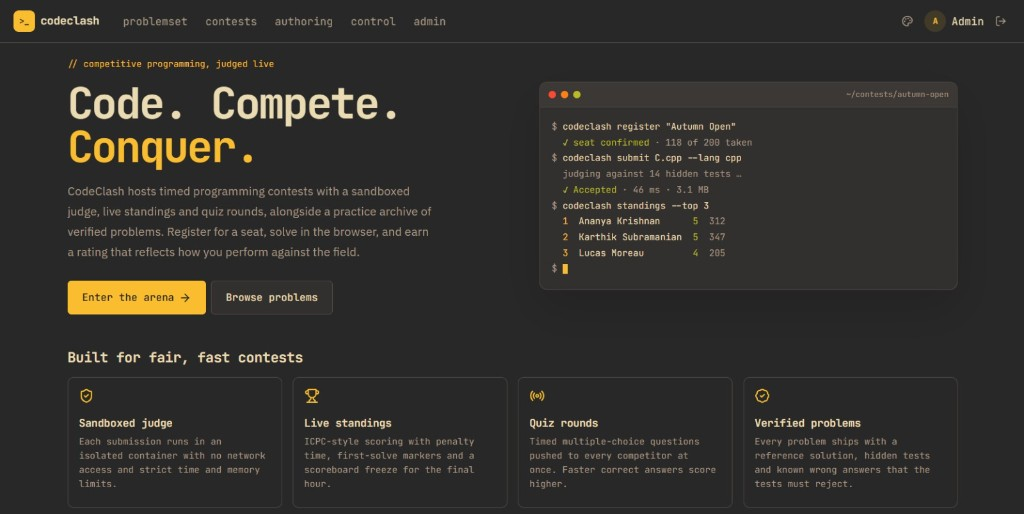
\includegraphics[width=\textwidth]{figures/home.jpg}
\caption{Landing page. The contest and quiz copy is ahead of the sprints that build them.}
\end{figure}

The problem set is \texttt{GET /api/archive}. The seed behind this screen has 146 problems and 33 tags. The chip row shows twelve tags and a control for the other twenty-one. ``Solved by'' is zero because no contest has published a standing.

\begin{figure}[ht]
\centering
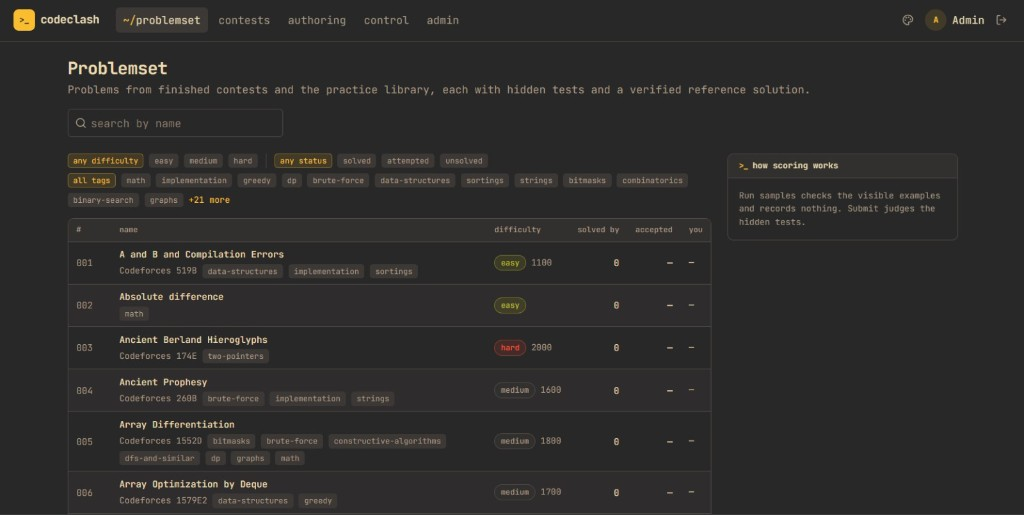
\includegraphics[width=\textwidth]{figures/problemset.jpg}
\caption{Practice archive. Run samples checks the visible examples and stores nothing. Submit is the judged path.}
\end{figure}

A correct solution of \emph{Cola} was submitted in Python~3 against a 2 second and 256\,MB limit, and the verdict came back Accepted. The editor lists C, C++17, Java, and Go as a later step. The program itself is case~8 below.

\begin{figure}[ht]
\centering
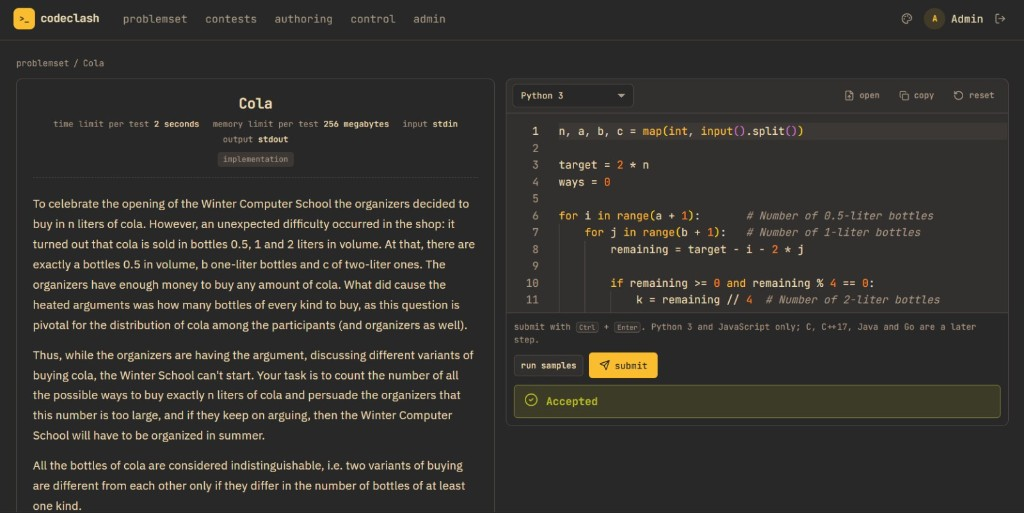
\includegraphics[width=\textwidth]{figures/submit.jpg}
\caption{Submit, then one verdict.}
\label{fig:submit}
\end{figure}

Behind Figure~\ref{fig:submit} the API checks that the email is verified, inserts the submission as queued, and appends it to the Redis stream. The judge claims it with a fresh token and runs it in its own container. The browser polls until \texttt{status} is \texttt{judged}.

\subsection{What we submitted}
\label{sec:sandbox}

These are the programs we sent through that same editor, one at a time. Practice limits are 2 seconds and 256\,MB. The container has no network, a read-only root, a process cap of 64, every capability dropped, and it runs as user \texttt{65534}. A program that catches the failure and exits normally would be scored Wrong Answer, so these ones let the failure stand.

\begin{pycase}{1. Infinite loop}{TLE}
while True:
    pass
\end{pycase}
The loop never prints an answer. The runner kills the container when the time limit is reached.

\begin{pycase}{2. Allocate 400 MB}{MLE}
x = bytearray(400 * 1024 * 1024)
print(len(x))
\end{pycase}
400\,MB is over the 256\,MB cap, so the allocation fails before the length is printed.

\begin{pycase}{3. Read a file outside the submission}{RE}
print(open("/codeclash-host-secret").read())
\end{pycase}
We first tried \texttt{/etc/passwd}. That file is inside the language image, so a successful read would not have shown that the host is hidden. This path is not in the image, and the open fails.

\begin{pycase}{4. Open a socket}{RE}
import socket
socket.create_connection(("1.1.1.1", 443), timeout=2)
print("connected")
\end{pycase}
``connected'' is never printed. The container is started with no network.

\begin{pycase}{5. One child process}{WA}
import subprocess
print(subprocess.run(
    ["echo", "sandbox-test"],
    capture_output=True, text=True, timeout=2).stdout)
\end{pycase}
A single child is allowed, and \texttt{echo} does run. The line it prints is not the sample answer, so the verdict is wrong answer rather than a blocked process. Case~7 is the one that hits the process cap.

\begin{pycase}{6. Flood standard output}{RE}
while True:
    print("x" * 10000)
\end{pycase}
The reason is ``output limit''. The flood is cut off before the 2 second limit.

\begin{pycase}{7. Keep forking}{RE or TLE}
import os
while True:
    os.fork()
\end{pycase}
The process cap is 64. The forks either hit that cap or run into the time limit.

\begin{pycase}{8. Cola, the accepted submit}{AC}
n, a, b, c = map(int, input().split())
target = 2 * n
ways = 0
for i in range(a + 1):       # 0.5-litre bottles
    for j in range(b + 1):   # 1-litre bottles
        remaining = target - i - 2 * j
        if remaining >= 0 and remaining % 4 == 0:
            k = remaining // 4  # 2-litre bottles
            if k <= c:
                ways += 1
print(ways)
\end{pycase}
This is the program in Figure~\ref{fig:submit}. Python~3, 2 seconds, 256\,MB, Accepted.

This set is pull request~\#7's isolation, exercised from the editor, while CC-35 is still waiting on authoring and a batch run.

\end{document}
